% IEEE standard conference template; to be used with:
%   spconf.sty  - LaTeX style file, and
%   IEEEbib.bst - IEEE bibliography style file.
% --------------------------------------------------------------------------

\documentclass[letterpaper]{article}
\usepackage{spconf,amsmath,amssymb,graphicx,epstopdf,url,float}
\usepackage{algpseudocode} 
\usepackage{algorithm}
\usepackage{mathtools}

\algnewcommand\algorithmicforeach{\textbf{for each}}
\algdef{S}[FOR]{ForEach}[1]{\algorithmicforeach\ #1\ \algorithmicdo}

\algdef{S}[FOR]{ForEachParallel}[1]{\algorithmicforeach\ #1\ \algorithmicdo \textbf{\ parallel} }

\algnewcommand{\LineComment}[1]{\State \(\triangleright\) #1}

\algnewcommand\True{\textbf{true}\space}
\algnewcommand\False{\textbf{false}\space}
\algnewcommand\Continue{\textbf{continue}\space}


% break URLs in bibtex references
\def\UrlBreaks{\do\/\do-}

% Example definitions.
% --------------------
% nice symbols for real and complex numbers
\newcommand{\R}[0]{\mathbb{R}}
\newcommand{\C}[0]{\mathbb{C}}

% bold paragraph titles
\newcommand{\mypar}[1]{{\bf #1.}}

% Title.
% ------
\title{Maximum Cardinality Matching for Bipartite Graphs}
%
% Single address.
% ---------------
\name{Thomas Meier, Isabelle Roesch, Conradin Roffler, Samuel Ueltschi} 
\address{Department of Computer Science\\ ETH Z\"urich\\Z\"urich, Switzerland}

\begin{document}
%\ninept
%
\maketitle
%

%The hard page limit is 6 pages in this style. Do not reduce font size
%or use other tricks to squeeze. This pdf is formatted in the American letter format, so the spacing may look a bit strange when printed out.

\begin{abstract}

We implement and optimize two existing parallel algorithms that solve the problem of maximum cardinality matching in bipartite graphs: Parallel Pothen Fan (PPF) and Parallel Tree Grafting (PTG). Our work is focused mainly on the analysis and possible optimizations of the PPF algorithm. We reason about the theoretical performance of PPF using the PRAM model and give a detailed description of the additional optimizations we implemented. We benchmark and test our implementations in a highly multi-threaded environment using a Xeon Phi multicore processor. The results confirm that our optimizations for PPF improve the original algorithm. 

\end{abstract}

\section{Introduction}\label{sec:intro}

Matching in bipartite graphs has several applications in computer science, for example the marriage problem or computing the block triangular 
form (BTF) of a sparse matrix \cite{Pothen:1990}.\\

Two recent publications by Azad et.\ al.\ are concerned with solving the bipartite maximum cardinality matching problem in parallel. 
The first paper~\cite{Azad:2012} presents a parallel version of the Pothen Fan algorithm (PPF) that achieves good performance 
on architectures with few fat cores. In the second paper~\cite{Azad:2015} a novel Parallel Tree Grafting (PTG) algorithm is presented 
that is designed to perform better on architectures with many thin cores. 
The authors of said paper also claim that PPF is not suited for architectures of this kind.\\

In this project we recreated some results of the original paper \cite{Azad:2012} by writing an implementation of PPF
that matches the performance stated in the original paper. We give detailed insight into our implementation and explain
implementation details and tricks that were omitted by the original authors of the algorithm. 
Our main contribution is a modified version of PPF that reduces the synchronization overhead of the original (see section \ref{sec:pfopt}).\\

We also implemented the PTG algorithm but were not able to reproduce the results of the original paper. 
Because we could not invest enough time to properly optimize the algorithm, we are not able to make any statements concerning the performance of this algorithm.
Nevertheless we give a brief introduction into PTG in section \ref{sec:tg}.\\

To verify the claim that PPF does not perform well on many thin cores, we conducted a series of experiments on the Xeon Phi platform~\cite{XeonPhi} (see section \ref{sec:exp}). 
Our experiments show that PPF does in fact scale well on this platform by using our improved version of PPF. We also discovered that PPF
performs especially well when starting with a bad initial matching (see section \ref{sec:exp}). 
By doing so, we achieved superlinear speedup for PPF on Xeon Phi.

\section{Background: Algorithms for Maximum Matching in Bipartite Graphs}\label{sec:background}

\mypar{Maximum Cardinality Matching in Bipartite Graphs}
Given a bipartite graph $G = (V = X \cup Y, E)$.
A matching $M[\cdot]: |V| \rightarrow |V| \cup \{v_{null}\}$ is a mapping that assigns each vertex $v$ a unique mate $M[v]$ s.t. 
$\forall v \in V.\ M[v] \neq v_{null} \implies v = M[M[v]] \wedge \{v, M[v]\} \in E$.
Each vertex can have at most one mate. A vertex $v$ is called matched iff $M[v] \neq v_{null}$. An edge is matched if its vertices are matched. 
We call a matching a maximum cardinality matching if it maximizes the number of edges expressed by $M$. See~\cite{intro_alg} for a detailed introduction.

\mypar{Augmenting Path based Algorithms}
The algorithms presented in this report are based on augmenting paths. 
There are other classes of algorithms for this problem, namely push-relabel~\cite{GoldbergT88} and auction based~\cite{Bertsekas}. 
These however are not the focus of this report. 

The best known sequential algorithm for bipartite maximum cardinality matching was discovered by Hopcroft and Karp~\cite{HK:1973}
and runs in $O(|E|\cdot \sqrt{|V|})$. Another algorithm which runs in $O(|E|\cdot|V|)$ was discovered by Pothen and Fan~\cite{Pothen:1990}.
Although this algorithm performs worse asymptotically than Hopcroft-Karp, in practice it performs better when parallelized according to Azad et.\ al.~\cite{Azad:2012}.

The core idea of both algorithms is to find so called augmenting paths. An augmenting path is a path where the first 
and last edge are unmatched and where the edges along the path alternate between matched and unmatched. 
An augmenting path can be inverted by adding every unmatched edge to the matching and removing every matched edge from the matching. 
This will increase the size of the matching by one. 
Augmenting path based algorithms try to find and invert such paths. If there are no more augmenting paths in a graph then the matching is maximal.

\mypar{Initial Matching}
Augmenting path based algorithms benefit from starting with an initial matching. 
A good algorithm for finding a suitable initial matching was discovered by Karp and Sipser~\cite{KarpS81}.
We use both Karp-Sipser and an augmented greedy version based on Karp-Sipser to get our initial matchings. 

\section{Algorithms and Optimizations}\label{sec:pfopt}

In this section, we describe the details of our PPF implementation and how we optimized it. In addition to that, we 
give a brief theoretical analysis of PPF using the PRAM model. Furthermore we also present our Tree Grafting implementation.

\subsection{Parallel-Pothen-Fan}\label{sec:pf}

\mypar{Implementation and Optimizations} Azad et.\ al.~\cite{Azad:2012} only give a very abstract description of their PPF implementation with no source code available. 
Coming up with an efficient PPF implementation proved to be challenging. 
In this section we describe our PPF implementation with a focus on the techniques used to match the performance of Azad et.\ al.\\

PPF computes the maximum cardinality matching by finding and inverting disjoint augmenting paths in parallel through multiple depth-first-searches (DFS)
that start from all unmatched vertices. A detailed explanation how PPF works can be found in \cite{Azad:2012}. 
Our implementation is given in \texttt{PPF} (see algorithm~\ref{alg:ppf}). 
Functionally, our algorithm description is equivalent to then one given by~\cite{Azad:2012} 
but goes into more detail and describes more optimizations than the original.\\

The main loop of \texttt{PPF} iteratively performs multiple DFS in parallel to find augmenting paths. 
When a path is found, it is inverted to increase the matching by one.
The description for this DFS is given in the recursive algorithm \texttt{FIND\_AND\_AUGMENT} (see algorithm~\ref{alg:fa}). 
Our DFS implementation finds a path and then inverts the matching while returning from the recursion. 
In practice, we use a stack based implementation of the recursive algorithm to avoid overflowing the stack as suggested by~\cite{Azad:2012}. 
Note that our algorithm only updates the matching of vertices on the right side of the graph ($M[y], y \in Y$). 
The left side ($M[x], x \in X$) can be updated later, when no more augmenting paths can be found. 
This saves unnecessary store instructions if an edge is added and removed from the matching multiple times.\\

Each thread locks the vertices it visits during the DFS. The original PPF uses a $visited$ array of atomic boolean flags to lock vertices. 
After each iteration, all flags in the $visited$ array are reset. This requires $O(|Y|)$ store instructions in the sequential phase of the algorithm. 
We solve this problem by storing the current iteration number in the $visited$ array when locking a vertex instead of just a flag. The iteration number is increasing, 
therefore we know that a vertex $v$ is unvisited if the value in $visited[v]$ is smaller than the current iteration. 
By using this technique, we were able to reduce the number of store instructions in the sequential phase of the algorithm from $O(|Y|)$ to $O(1)$.\\

Because all threads read and write the $visited$ array in parallel, read and store operations must be performed atomically to guarantee correctness. 
This is a large bottleneck of the algorithm because threads have to wait for the store operations of other threads to complete. 
In the original algorithm by Azad et.\ al.~\cite{Azad:2012}, Test-and-Set is used to set the flags in the $visited$ array. 
An equivalent implementation of this approach applied to our algorithm is given in \texttt{$CLAIM_{TAS}$} (see algorithm~\ref{alg:claim_tas}). 
Using Test-and-Set is problematic because it adds an unnecessary overhead to each failed attempt of locking a vertex when there is no data race. 
We solve this issue by using the Test-and-Test-and-Set approach to lock vertices (see \texttt{$CLAIM_{TTAS}$} in algorithm~\ref{alg:claim_ttas}).
Before using an atomic operation to lock a vertex, we first try a regular memory load. If the vertex is already locked we can omit the atomic operation. 
This has the benefit of increased caching possibilities and reduced memory traffic. 
We experimentally verified that PPF performs better with Test-and-Test-and-Set than with Test-and-Set in section \ref{sec:exp}.

The source code of our PPF implementation is available online\footnote{\url{https://github.com/suem/dphpc-project/blob/master/src/ppf3.cpp}} for further reference.\\

\begin{algorithm}
    \caption{Parallel Pothen Fan}
    \label{alg:ppf}
    \begin{algorithmic}[1]
        \Procedure{PPF}{$G=(V=X \cup Y,E), M$}

        \LineComment{Initialization}
        \State $lookahead[x] \gets \text{first neighbor of x}$ \Comment{$x \in X$}
        \State $iter \gets 0$
        \State $visited[y] \gets iter$ \Comment{$y \in Y$}
        \State $unmatched \gets \{x \in X, x \ \text{unmatched}\}$

        \LineComment{Discover augmenting paths}
        \Repeat 
            \State $iter \gets iter + 1$        
            \State $path\_found \gets \False$        
        \ForEachParallel{$x \in unmatched$}
            \If {$x$ matched}
                \State \Continue \Comment{skip $x$ if already matched}
            \EndIf
            \State $found \gets find\_and\_augment(x)$        
            \If {found}
                \State $path\_found \gets \True$        
            \EndIf
        \EndFor
        \Until{$path\_found = \False$}

        \LineComment{Complete matching}
        \ForEachParallel{$y \in Y$, $y$ matched}
            \State $M[M[y] \gets y$        
        \EndFor
        
        \EndProcedure
    \end{algorithmic}
\end{algorithm}


\begin{algorithm}
    \caption{Find and Augment}
    \label{alg:fa}
    \begin{algorithmic}[1]
        \Procedure{find\_and\_augment}{$x$}

            \LineComment{Lookahead Step}

            \ForEach{$y \in adj[x]$, starting at $lookahead[x]$}
                \State $lookahead[x] \gets \text{next neighbor of}\ x$
                \If {$y$ is unmatched}
                    \If {$CLAIM_{TTAS}(y)$}
                        \State $M[y] \gets x$ \Comment{make $x$ the mate of $y$}
                        \State \textbf{return} \True
                    \EndIf
                \EndIf
            \EndFor
            
            \LineComment{Recursive Path Search}
            \ForEach{$y \in adj[x]$}
                \If {$CLAIM_{TTAS}(y)$}
                    \State $success \gets find\_and\_augment(M[y])$
                    \If {$success$}
                        \State $M[y] \gets x$ \Comment{make $x$ the mate of $y$}
                        \State \textbf{return} \True
                    \EndIf
                \EndIf
            \EndFor
        \EndProcedure
    \end{algorithmic}
\end{algorithm}

\begin{algorithm}
    \caption{Claim with Test-and-Set}
    \label{alg:claim_tas}
    \begin{algorithmic}[1]
        \Procedure{$CLAIM_{TAS}$}{$y$}
            \State $y\_iter \gets atomic\_exchange(visited[y], iter)$
            \State \textbf{return} $y\_iter < iter$
        \EndProcedure
    \end{algorithmic}
\end{algorithm}


\begin{algorithm}
    \caption{Claim with Test-and-Test-and-Set}
    \label{alg:claim_ttas}
    \begin{algorithmic}[1]
        \Procedure{$CLAIM_{TTAS}$}{$y$}
            \If {$visited[y] < iter$}
                \State $y\_iter \gets atomic\_exchange(visited[y], iter)$
                \State \textbf{return} $y\_iter < iter$
            \EndIf
            \State \textbf{return} \False
        \EndProcedure
    \end{algorithmic}
\end{algorithm}

\mypar{PRAM Analysis} The original authors of PPF did not provide a theoretical analysis of the runtime of the algorithm.
Doing such an analysis is non-trivial as the runtime of the algorithm mainly depends on the structure of the provided
input graph. If a graph has many non overlapping augmenting paths, then PPF performs well as there are no inter-thread conflicts. 
However if there are many overlaps then the threads will block each other often and the algorithm can only make little progress.
In this section we give a brief analysis of PPF using the PRAM model to illustrate the average parallelism of PPF for the best and worst case
scenario. \\

The work PPF has to perform is $O(|V|\cdot|E|)$. Finding an augmenting path requires a DFS of length at most $|E|$. 
This has to be performed for all $|V|$ vertices. Note that PPF might perform useless work that does not contribute to the solution
if it is blocked by another thread and has to abort the DFS. 
The PTG algorithm described in section \ref{sec:tg} attempts to mitigate this problem.\\

Figure~\ref{fig:pram} illustrates the two program DAGs of PPF for the best case scenario (left) and the worst case scenario (right).

In the best case scenario, the input graph only consists of non-overlapping augmenting paths, which can then all be found in parallel without conflicts. 
This is illustrated by the vertical gray node paths in the DAG.
Therefore the maximal depth of the DAG is $|E|$, matching the length of a DFS. Hence PPF has an average parallelism of $O(|V|)$ in the best case.

In the worst case scenario, the input graph consists of augmenting paths that always overlap. 
In this case, only one thread will succeed per iteration and the other threads cannot perform any work. 
Unsuccessful threads are indicated by the white nodes on the DAG on the right. 
Therefore the depth of the DAG is the same as the work because there is no parallel work, resulting in an average parallelism of $O(1)$.\\

\begin{figure}\centering
  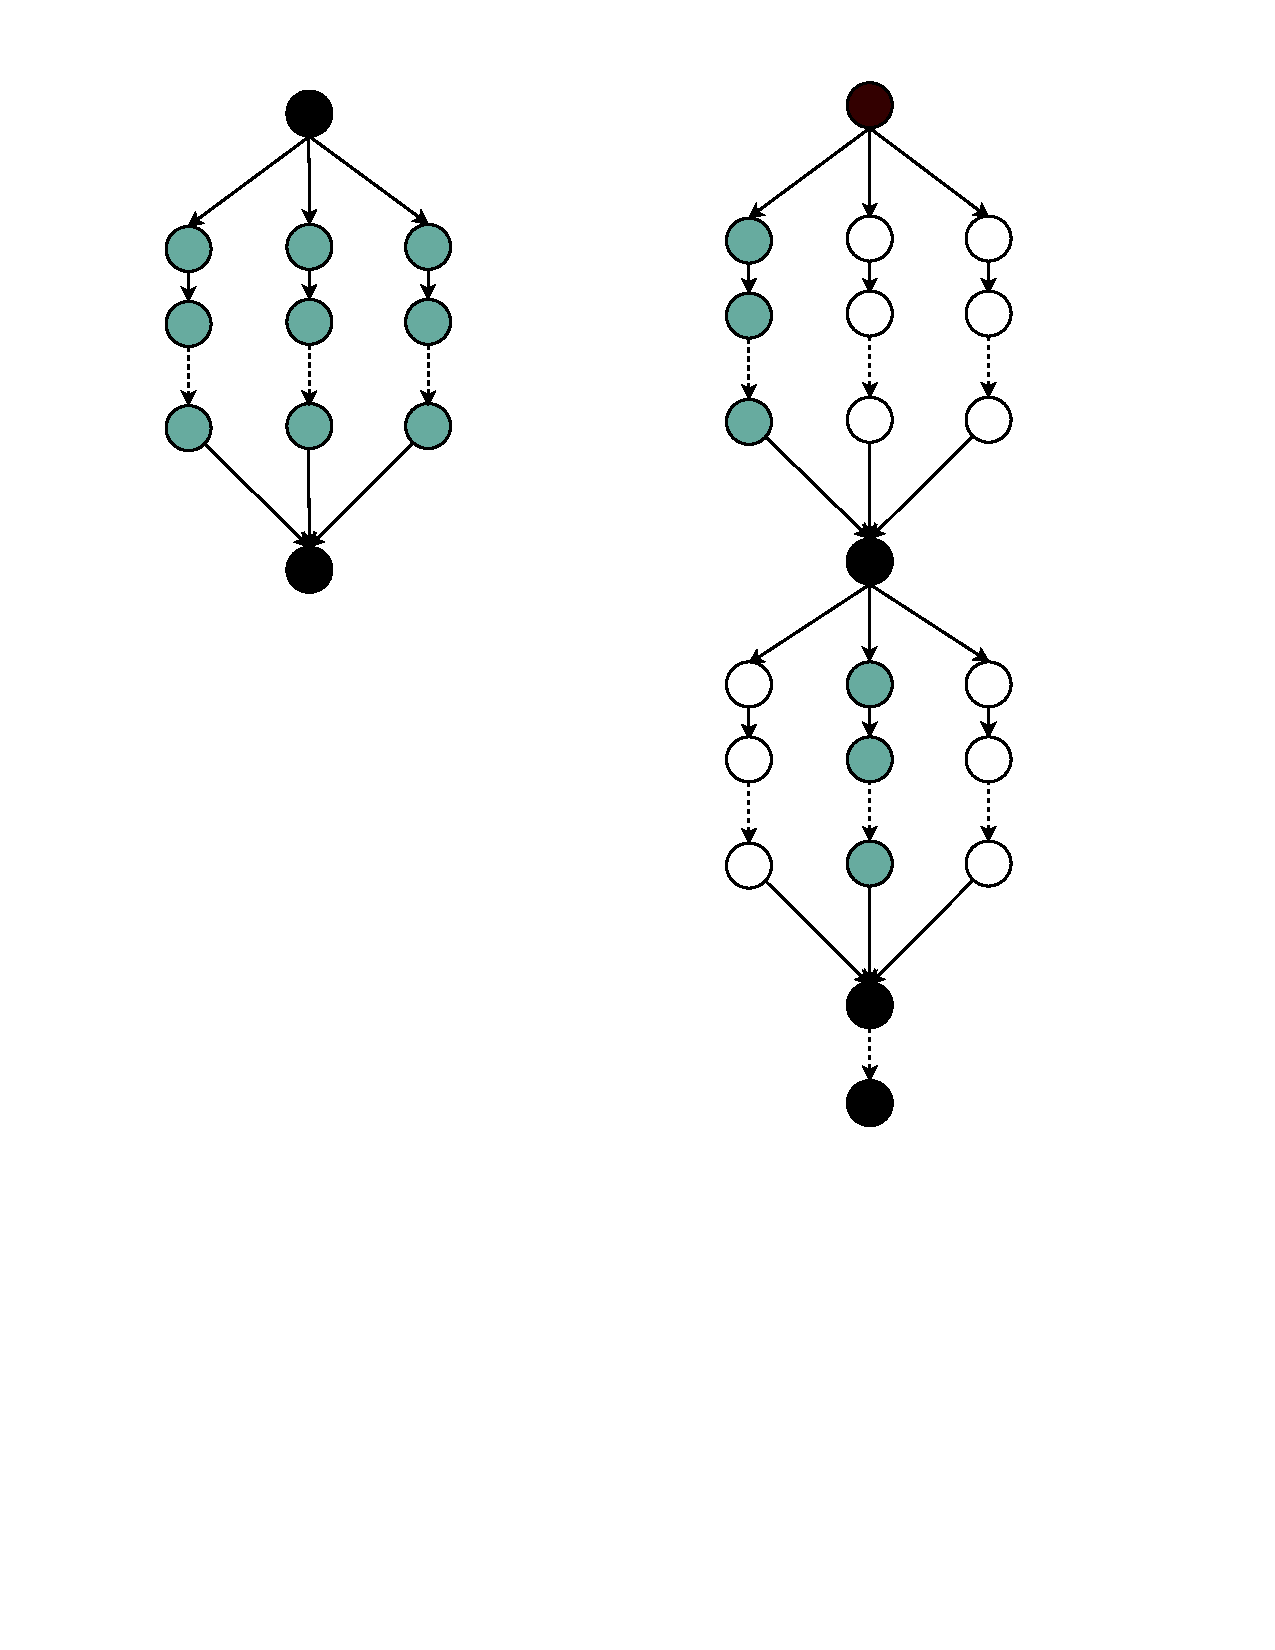
\includegraphics[height=5cm, trim={2.5cm 8cm 4cm 1cm}, clip]{PRAM.pdf}
  \caption{DAG for PRAM analysis of PPF. Worst case scenario on the right, best case scenario on the left.}
  \label{fig:pram}
\end{figure}

The average parallelism of PPF lies between $O(1)$ and $O(|V|)$ depending on the input graph. 
In section \ref{sec:exp} we show that for real-world input data PPF achieves a speedup that is close to the optimal average parallelism.

\subsection{Tree Grafting}\label{sec:tg}

The second algorithm we examined that solves the problem of maximum matching on bipartite graphs is the Tree Grafting algorithm, as described in \cite{Azad:2015}. One of the paper's claims is that Tree Grafting performs better than PPF on architectures with many thin cores such as the Xeon Phi. \\
We give a short overview of the algorithm we have implemented and on the optimizations we did. \\

\mypar{Parallel Tree Grafting} 
The Parallel Tree Grafting algorithm (PTG) takes a bipartite graph and an initial matching $M$ as input and returns a maximum matching by updating $M$.
PTG is - like PPF - a multi-source searching algorithm. It starts to search for augmenting paths from different unmatched vertices and constructs a forest of alternating trees.\\
The main difference between PPF is the reuse of already found trees. PPF forgets about the trees it previously found but could not use and has to reconstruct them in every new iteration.\\
PTG however keeps track of augmenting trees which can still be extended (active trees) and then grafts other trees to the active trees to prolong the augmenting paths contained in them.\\
For a more detailed explanation of the PTG algorithm including pseudocode, see \cite{Azad:2015}.\\

\mypar{Optimizations}
Our implementation of the PTG algorithm follows the implementation described in the paper very closely. To build the augmenting paths, we have used the same optimizations as already described in our optimized version of PPF. To store the pointers to the root, leaf and other nodes the PTG algorithm utilizes, we have implemented our own version of a non-blocking queue as a data structure. \\

The source code of our PTG implementation is available online\footnote{\url{https://github.com/suem/dphpc-project/blob/master/src/tree_grafting.cpp}} for further reference.


\section{Experimental Results}\label{sec:exp}

In this section we explain the benchmarking process. We first describe the experimental setup on which we perform our benchmarks on. Then we explain the input data we use. We then proceed to describe which test cases we benchmark. Finally, we discuss the results from our benchmarks.\\
%Here you evaluate your work using experiments. You start again with a
%very short summary of the section. The typical structure follows.

\mypar{Experimental Setup} 
%Specify the platform (processor, frequency, maybe OS, maybe cache sizes)
%as well as the compiler, version, and flags used. If your work is about performance, 
%I strongly recommend that you play with optimization flags and consider also icc for additional potential speedup.
We execute our benchmarks on an Intel Xeon Phi coprocessor (7120 Series) which is based on the Intel MIC architecture. The Xeon Phi has a total of 61 cores which run at a frequency of 1.24 GHz. Each core can run up to four threads, which gives us a total of 244 threads. The Xeon Phi coprocessor has a fully coherent L2 cache with a size of 30.5 MB. To compile our code we use the Intel \texttt{icpc} compiler with the following flags: \texttt{-openmp, -std=c++11, -Wall, -O3, -mmic, -lrt}.\\
% Xeon Phi (5110P), GCC, -O3, 60 simplified Intel CPU cores running at 1056 MHz and supports 4 threads  per core, resulting in a total of 240 threads. Each core has a 32kb L1 data cache, a 32kb L1 instruction cache and a private 512 kb L2 unified cache. \cite{Ramos:2013}

%Then explain what kind of benchmarks you ran. The idea is to give enough information so the experiments are reproducible by somebody else on his or her code.
%For sorting you would talk about the input sizes. For a tool that performs NUMA optimization, you would specify the programs you ran.

\mypar{Test Data}
To test our algorithms, we use several real world graphs from the SuiteSparse Matrix Collection\footnote{\url{http://www.cise.ufl.edu/research/sparse/matrices}}.
The graphs and their attributes are listed in table \ref{table:testdata}. 
To convert regular graphs to bipartite graphs, we applied the same technique as described in \cite{Azad:2015}. 
Let $M$ be the $m \times n$ adjacency matrix of an input graph. 
The corresponding bipartite graph $G = (V = X \cup Y, E)$ is defined as $X = \{x_1, \dots, x_m\}$, $Y = \{y_1, \dots, y_n\}$ and $\{x_i, y_j\} \in E \iff M_{ij} \neq 0$.\\


\\
\begin{table}
\centering
\begin{tabular}{ |l|l|l|l| }
\hline
 & $\lvert V \rvert$ & $\lvert E \rvert$ & Density \\ \hline
coPaperDBLP & 1'080'872 & 15'245'732 & $5.22\mathrm{e}{-5}$ \\ \hline
Wikipedia & 7'030'396 & 45'030'392 & $3.64\mathrm{e}{-6}$ \\ \hline
Amazon0312 & 801'454 & 3'200'440 & $1.99\mathrm{e}{-5}$ \\ \hline
Gnutella & 73'364 & 176'656 & $1.31\mathrm{e}{-4}$ \\ \hline
\end{tabular}
\caption{Test data used for benchmarks. $\lvert V \rvert$ is the number of vertices, $\lvert E \rvert$ the number of edges. The density describes the sparseness of the graph, where $0.0$ represents an empty graph and $1.0$ a fully connected bipartite graph.}
\label{table:testdata}
\end{table}

\mypar{Benchmarks}
We measure the execution times of the algorithms specified in section \ref{sec:pfopt} on different graphs and with different initial matchings. We compare the execution times of the different algorithms for three reasons: To verify the impact of our optimizations, to reproduce the results of \cite{Azad:2012} and \cite{Azad:2015}, and to observe the impact of different initial matchings on the execution times. As a baseline for the speedup we use the sequential Pothen-Fan algorithm executed on a single core of the Xeon Phi.\\

\mypar{Verification}
In order to verify the correctness of our implementations, we compare our results to the size of a matching obtained with the \textit{Edmonds Maximum Cardinality Matching} algorithm \cite{BoostEdmonds} from the Boost Graph library.\\


\begin{figure}\centering
	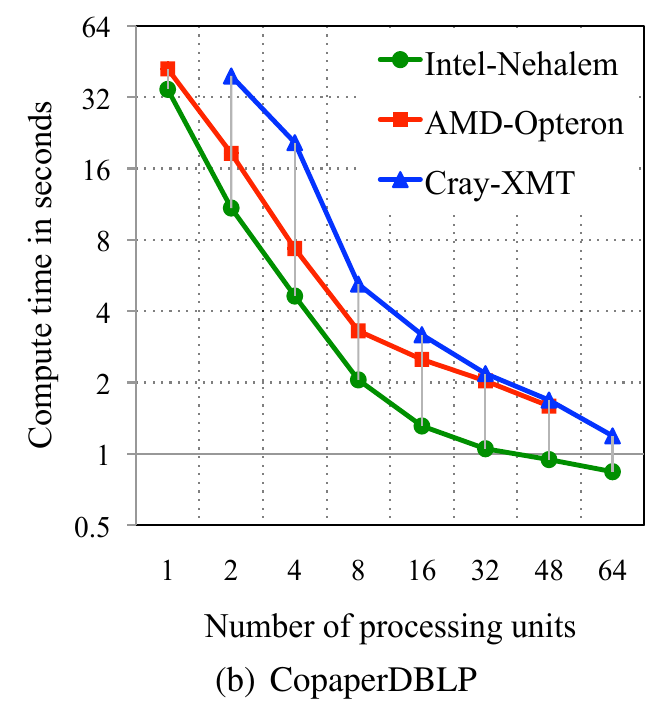
\includegraphics[width=5cm]{../../plot/output/report/coPaperAzadPlot.png}
    \caption{Runtimes of PPF on coPaperDBLP graph. Plot taken from original paper \cite{Azad:2012}.}
	\label{fig:azadCopaper}
\end{figure}


\begin{figure}\centering
	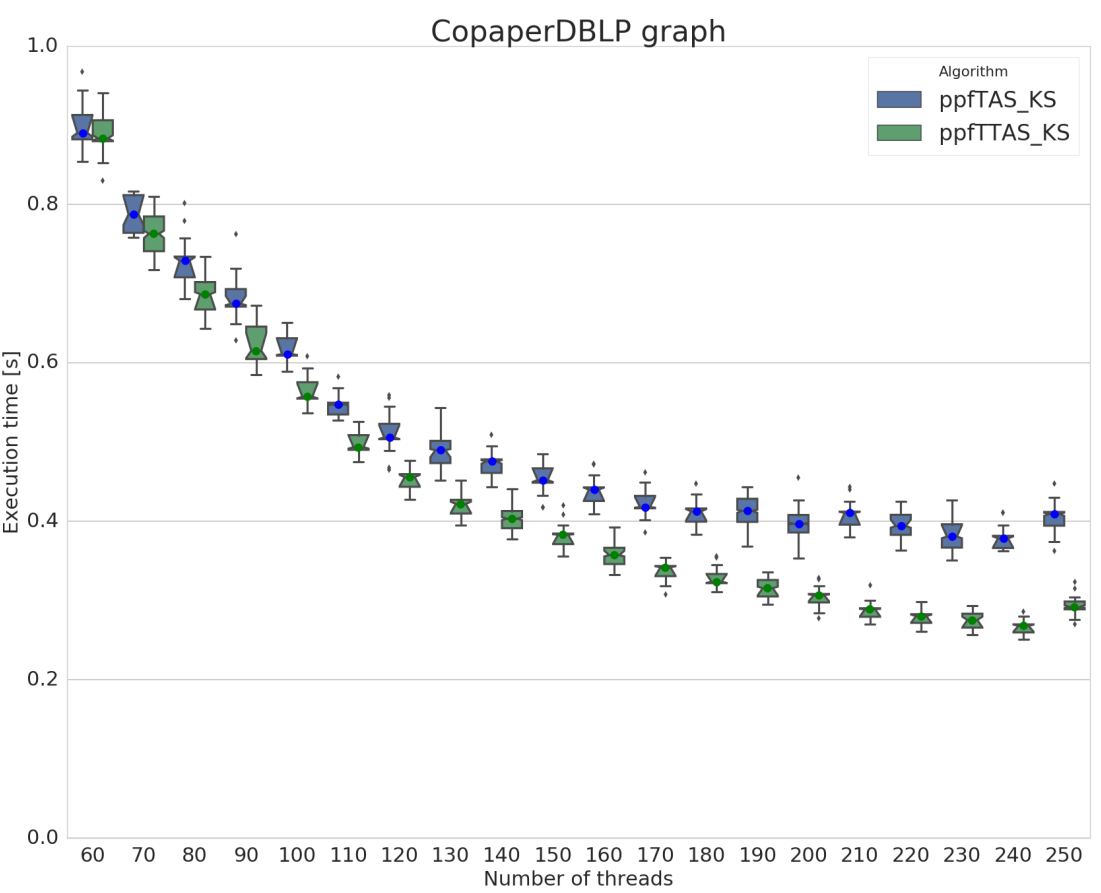
\includegraphics[width=8.3cm]{../../plot/output/report/coPaperDBLP_PPFTASvsPPFTTAS.png}
	\caption{Execution time of the PPF implementation from Azad et al. compared with the execution time of the optimized implementation introduced in this report. Both implementations use the Karp-Sipser heuristic for the initial matching.}
	\label{fig:tasvsttas}
\end{figure}


\mypar{Results} First, we compare the PPF implementation from Azad et al. with our optimized implementation. 
Figure~\ref{fig:azadCopaper} shows the runtime of the original PPF implementation on the coPaperDBLP graph. 
We ran our implementation on the same graph, once with Test-and-Set and once with Test-and-Test-and-Set (see figure \ref{fig:tasvsttas}). 
Even though the two experiments were conducted on different architectures, we can nevertheless observer that the achieved runtimes are in the same area. 
This supports our claim that we were able to match the performance achieved in \cite{Azad:2012}. 
We were even able to beat the original in terms of absolute runtime.
Furthermore, as figure \ref{fig:tasvsttas} demonstrates, we can see that our proposed improvement to PPF using Test-and-Test-and-Set performs 
better as the number of cores increases. The reason for this is that with a higher number of threads working on the graph, 
the contention on the $visited$ array is higher and thus \texttt{$CLAIM_{TAS}$} invalidates a cache-line with each unsuccessful attempt to lock a vertex.\\
 
\begin{figure}\centering
	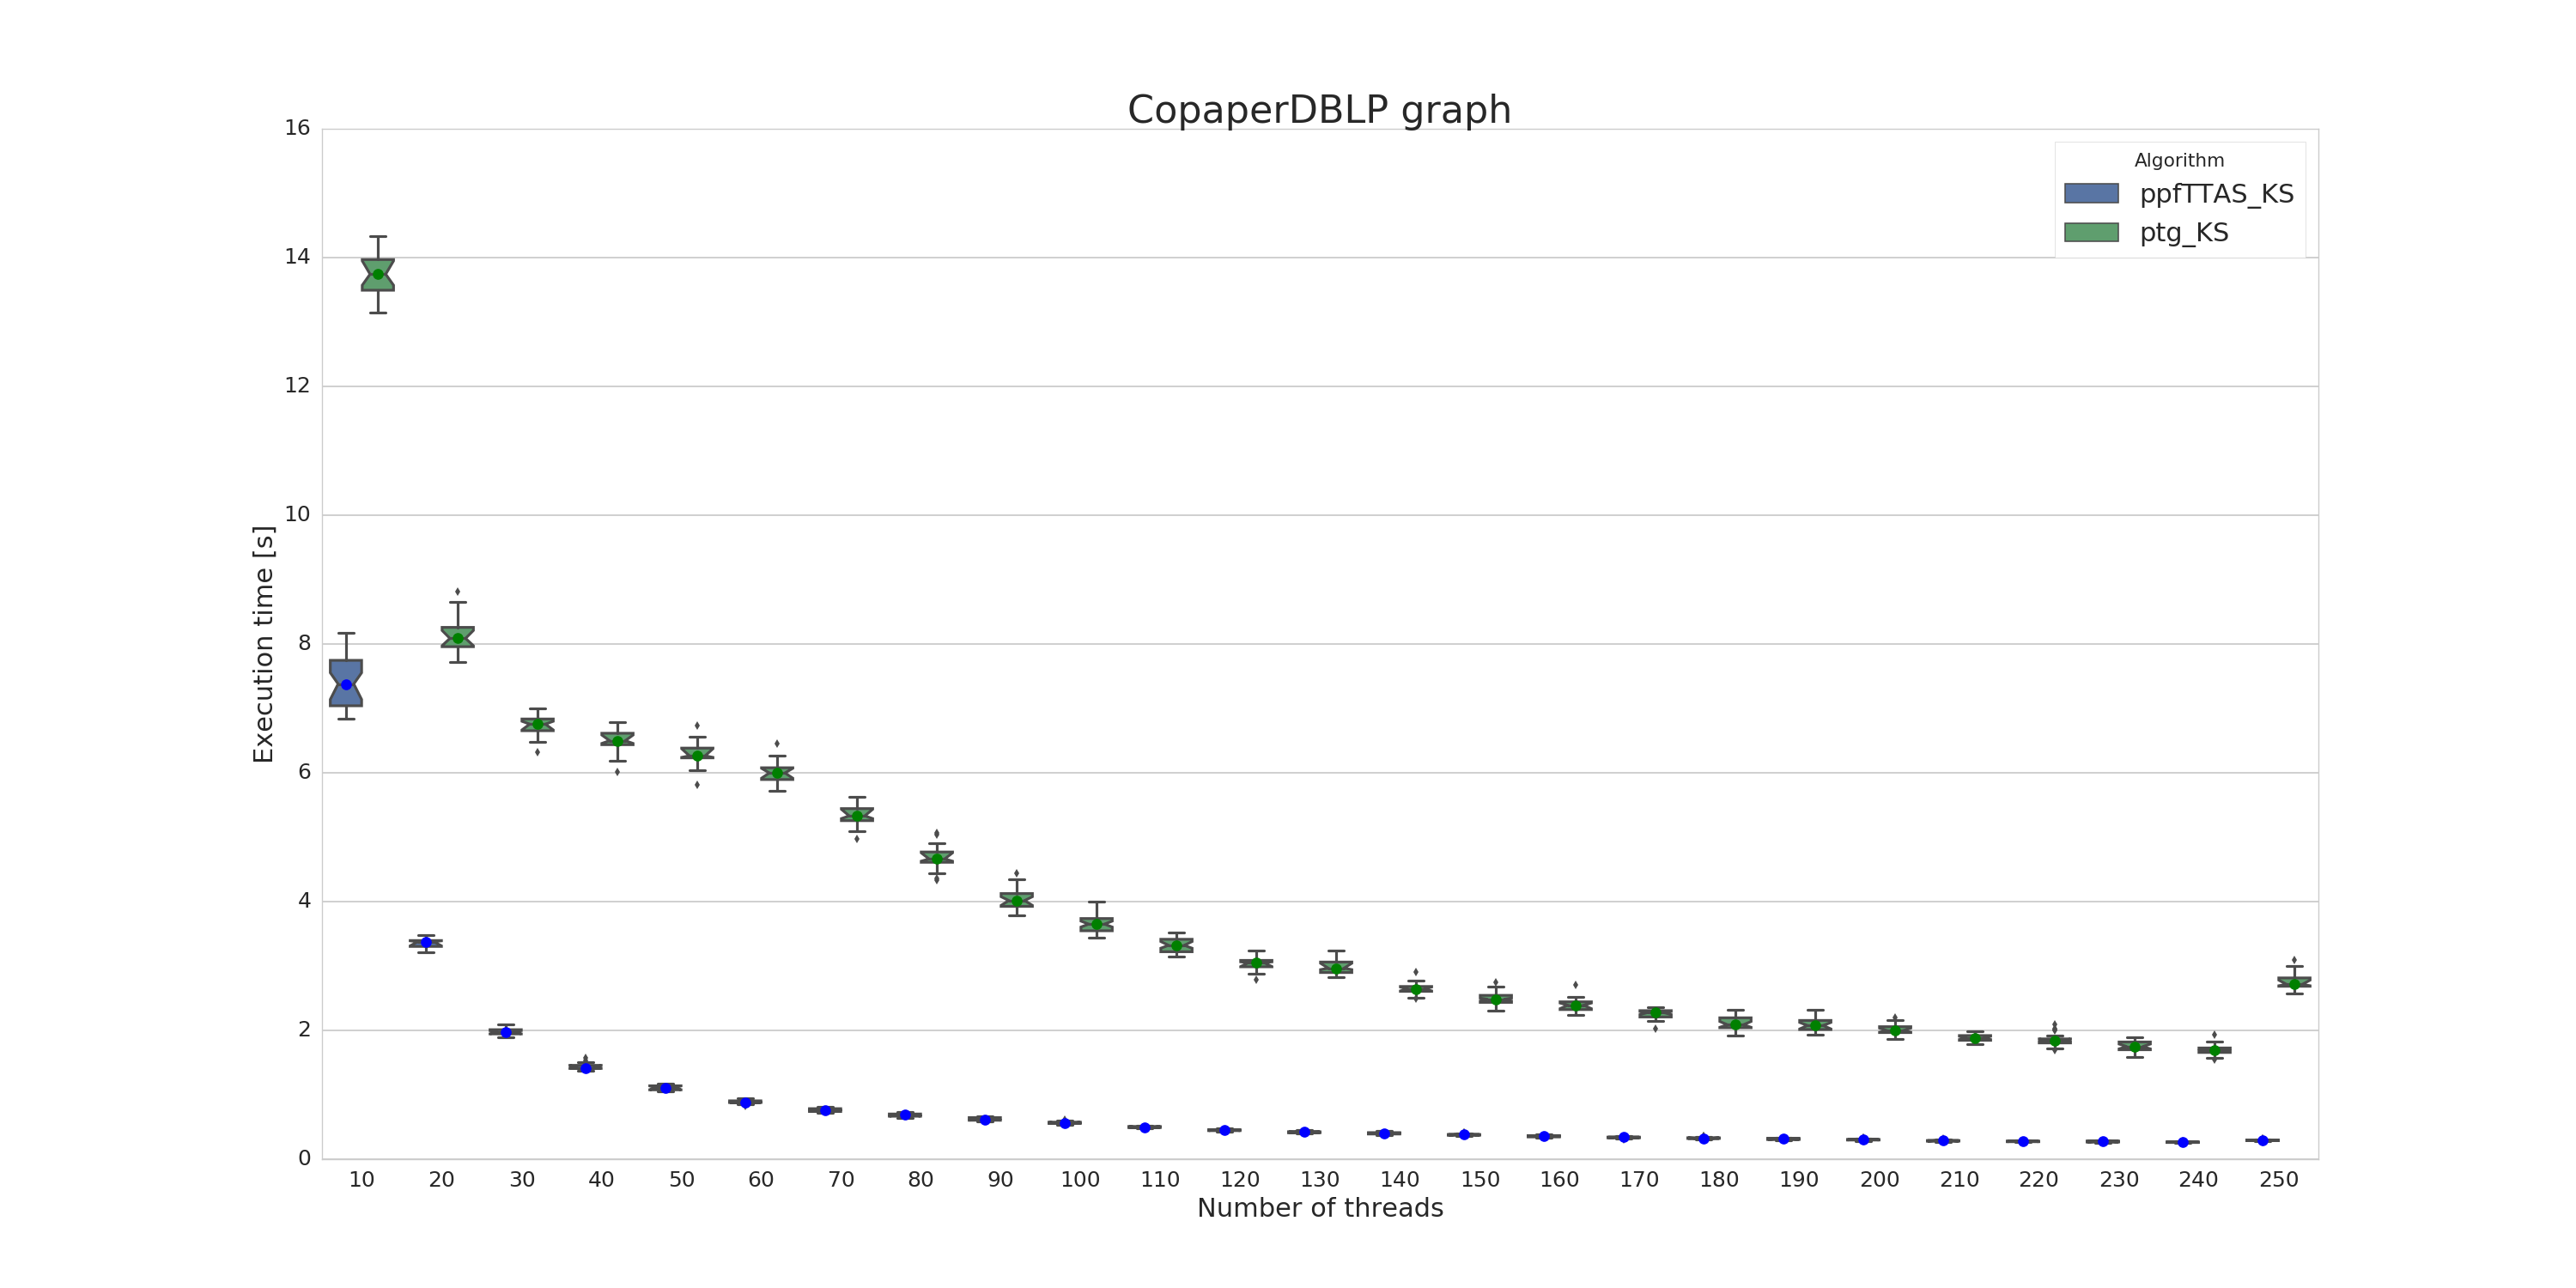
\includegraphics[width=8.3cm]{../../plot/output/report/coPaperDBLP_TGvsPPFTTAS.png}
	\caption{Execution time of our PTG implementation compared with our PPF implementation. Both implementations use the Karp-Sipser heuristic for the initial matching.}
	\label{fig:tgvsppf}
\end{figure}

Next, we compare our implementation of the PTG algorithm with our implementation of the PPF algorithm on the coPaperDBLP graph (figure \ref{fig:tgvsppf}). As we can see, even though the PTG algorithm scales up to 240 threads, it is still outperformed by the PPF algorithm. As a consequence of that, we cannot confirm the claim of Azad et al. that the PTG algorithm is better suited for an architecture with many thin cores than the PPF algorithm. A possible reason for this would be that our PTG implementation is not optimal.\\

\begin{figure}\centering
	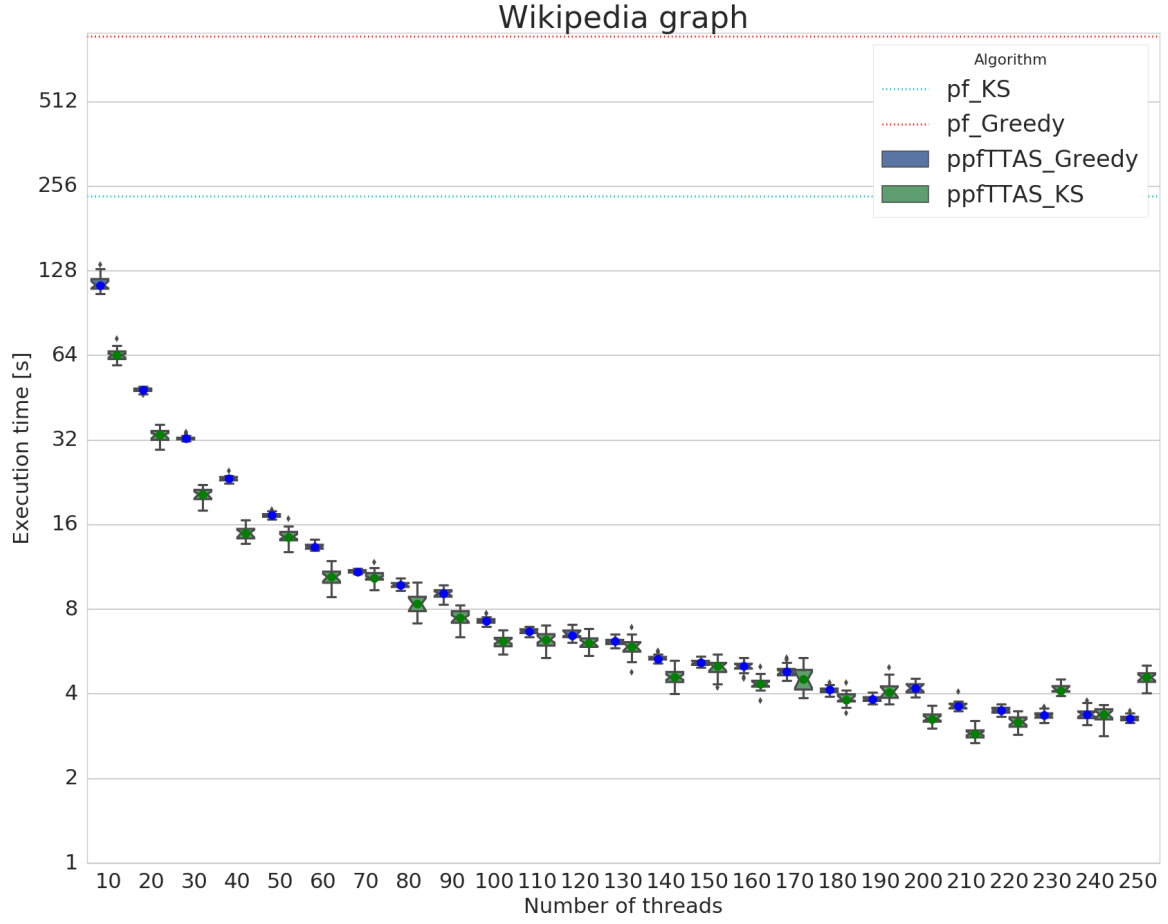
\includegraphics[width=8.3cm]{../../plot/output/report/wikipedia_PFvsPPFTTAS.png}
	\caption{Execution times of our PF and PPF implementations using both the Karp-Sipser and the Greedy initial matching.}
	\label{fig:ksvsgreedy}
\end{figure}
%TODO Insert matching sizes

Finally, we look at how the initial matching impacts the performance of our PPF implementation. 
Figure \ref{fig:ksvsgreedy} shows the execution times of our PPF implementation using both the Greedy (91\% optimal) and the Karp-Sipser (99\% optimal) initial matching,
as well as the corresponding execution times for sequential PF. 
The quality of the initial matching has a large impact on the sequential version of the algorithm. 
For PPF however, the difference vanishes with an increasing number of threads. 
This leads to a substantial difference in the speedup, as we can see in figure \ref{fig:ksvsgreedy_s}. 

\begin{figure}
	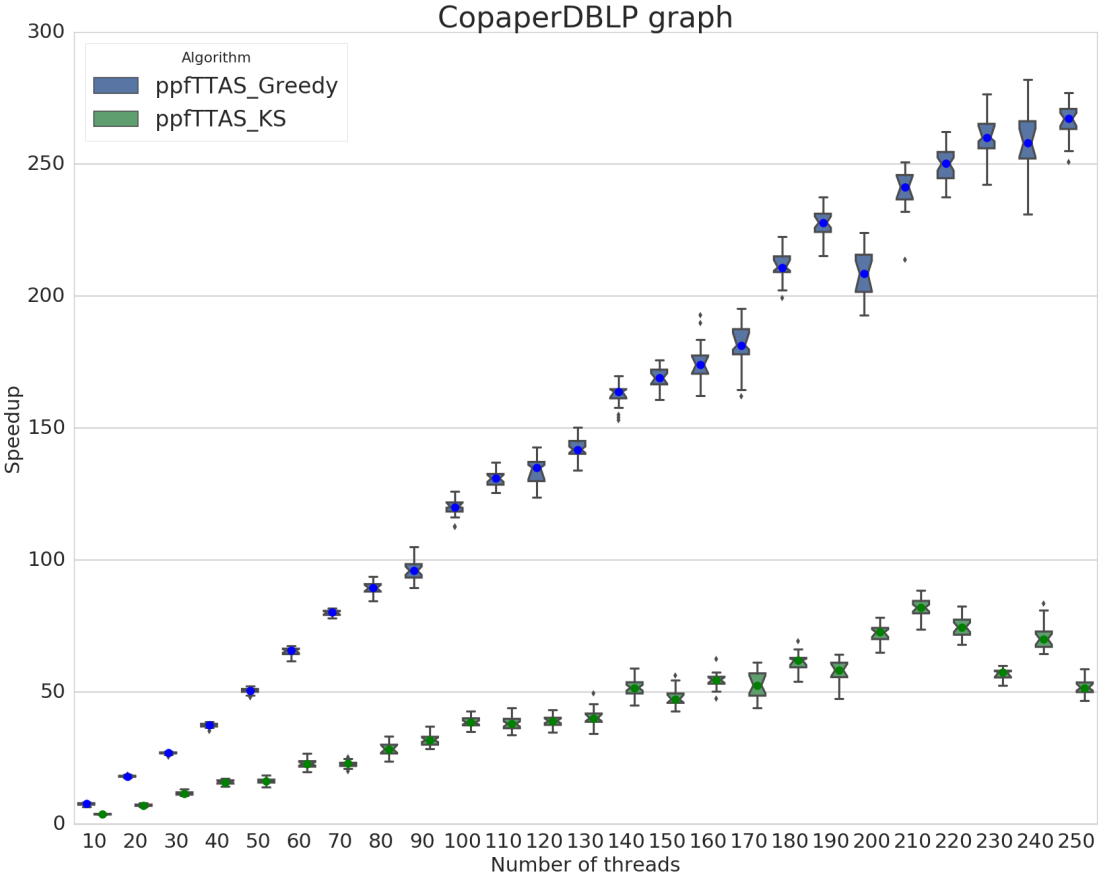
\includegraphics[width=8.3cm]{../../plot/output/report/wikipedia_GREEDYvsKS.png}
	\caption{Speedups of our PPF implementation using both the Karp-Sipser and the Greedy initial matching. The baseline is the sequential PF using the respective initial matching.}
	\label{fig:ksvsgreedy_s}
\end{figure}

%Next divide the experiments into classes, one paragraph for each. In each class of experiments you typically pursue one questions that then is answered by a suitable plot or plots. For example, first you may want to investigate the performance behavior with changing input size, then how your code compares to external benchmarks.
%
%For some tips on benchmarking including how to create a decent viewgraph see pages 22--27 in \cite{Pueschel:10}.

%{\bf Comments:}
%\begin{itemize}
%\item Create very readable, attractive plots (do 1 column, not 2 column plots
%for this report) with readable font size. However, the font size should also not be too large; typically it is smaller than the text font size.
%An example is in Fig.~\ref{fftperf} (of course you can have a different style).
%\item Every plot answers a question. You state this question and extract the
%answer from the plot in its discussion.
%\item Every plot should be referenced and discussed.
%\end{itemize}
%
%\begin{figure}\centering
%  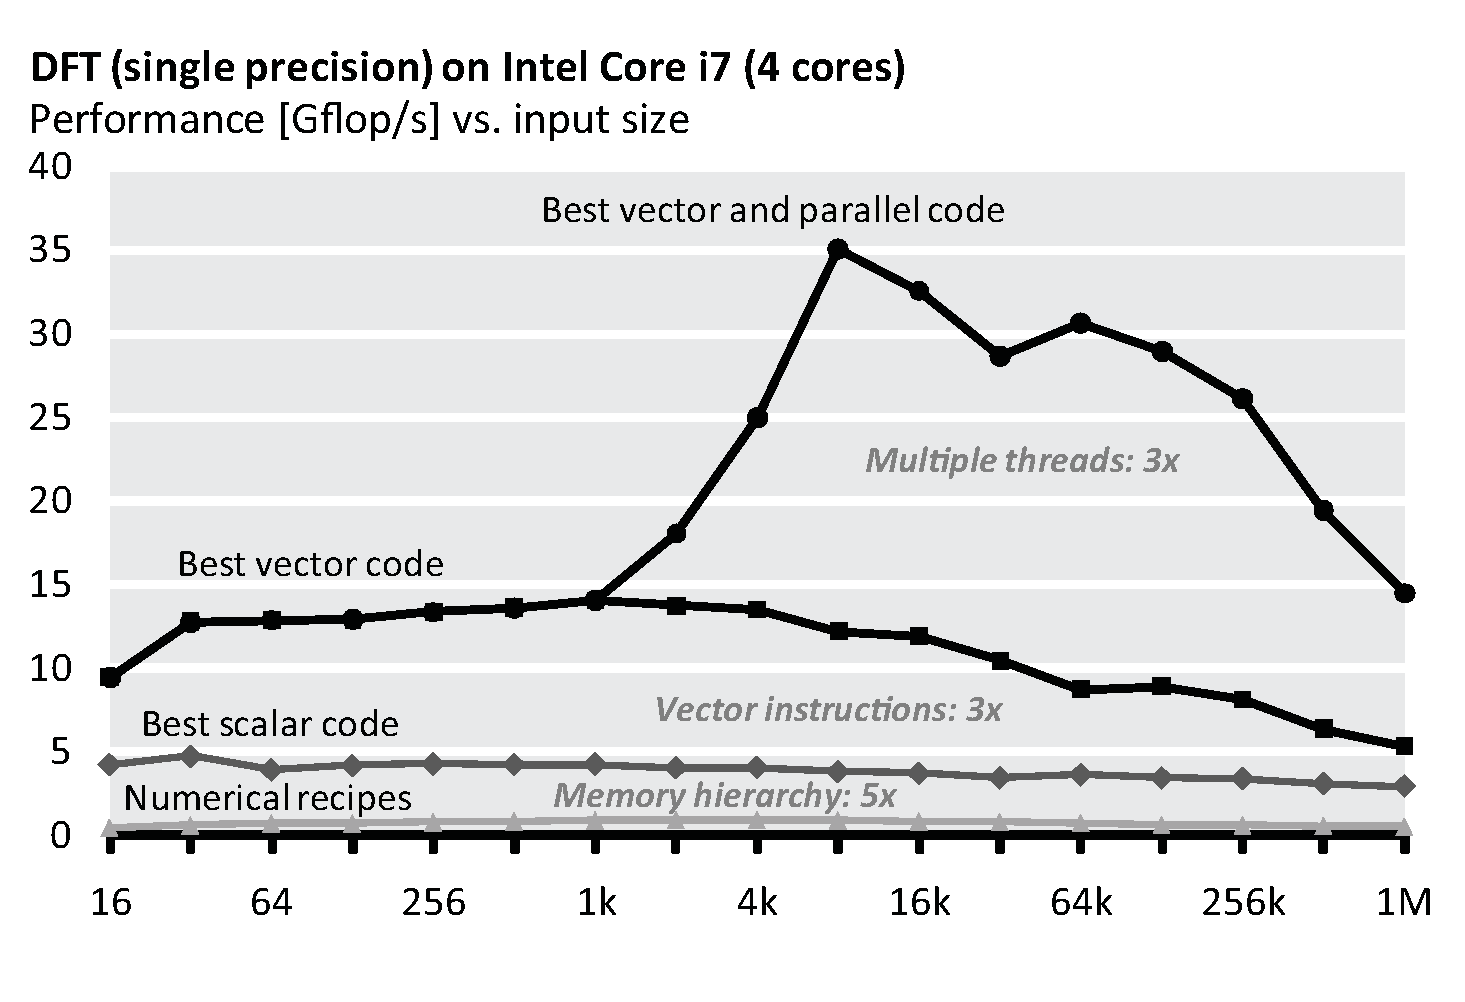
\includegraphics[scale=0.33]{dft-performance.eps}
%  \caption{Performance of four single precision implementations of the
%  discrete Fourier transform. The operations count is roughly the
%  same. The labels in this plot are maybe a little bit too small.\label{fftperf}}
%\end{figure}

\section{Conclusions}

We analyzed and implemented the PPF algorithm, building upon the pseudocode provided in the original paper~\cite{Azad:2012}. We then designed and evaluated new optimizations for the PPF algorithm, which resulted in performance benefits over the original implementation. Our experimental results show that our approach using Test-and-Test-and-Set to lock a vertex outperforms the  Test-and-Set approach used in the original PPF algorithm by Azad et.\ al.\ \cite{Azad:2012}. Using a more clever way to update the \textit{visited} array further improved the runtime of the algorithm.\\

The claim of Azad et.\ al. \cite{Azad:2015} that PPF is not well suited for architectures with many thin cores could not be verified by our experiments on the Xeon Phi multicore processor. Our optimized PPF implementation yields a superlinear speedup compared to the sequential PF implementation and scales up to 240 threads. We have to mention however that the superlinear speedup is also due to caching effects on the Xeon Phi. The sequential PF algorithm only runs on a single core which is very weak compared to the resources of all cores combined.\\

While our implementation of the PTG algorithm also scales up to 240 threads, it is still an order of magnitude slower than our PPF implementation, independent of the number of threads used. We could thus not confirm that PTG is an improvement over PPF.

%
%Here you need to summarize what you did and why this is
%important. {\em Do not take the abstract} and put it in the past
%tense. Remember, now the reader has (hopefully) read the report, so it
%is a very different situation from the abstract. Try to highlight
%important results and say the things you really want to get across
%such as high-level statements (e.g., we believe that .... is the right
%approach to .... Even though we only considered x, the
%.... technique should be applicable ....) You can also formulate next
%steps if you want. Be brief. After the conclusions there are only the references.
%
%\section{Further comments}
%
%Here we provide some further tips.
%
%\mypar{Further general guidelines}
%
%\begin{itemize}
%\item For short papers, to save space, I use paragraph titles instead of
%subsections, as shown in the introduction.
%
%\item It is generally a good idea to break sections into such smaller
%units for readability and since it helps you to (visually) structure the story.
%
%\item The above section titles should be adapted to more precisely
%reflect what you do.
%
%\item Each section should be started with a very
%short summary of what the reader can expect in this section. Nothing
%more awkward as when the story starts and one does not know what the direction is or the goal.
%
%\item Make sure you define every acronym you use, no matter how
%convinced you are the reader knows it.
%
%\item Always spell-check before you submit (to us in this case).
%
%\item Be picky. When writing a paper you should always strive for very
%high quality. Many people may read it and the quality makes a big difference.
%In this class, the quality is part of the grade.
%
%\item Books helping you to write better: \cite{Higham:98} and \cite{Strunk:00}.
%
%\item Conversion to pdf (latex users only): 
%
%dvips -o conference.ps -t letter -Ppdf -G0 conference.dvi
%
%and then
%
%ps2pdf conference.ps
%\end{itemize}

%\mypar{Graphics} For plots that are not images {\em never} generate the bitmap formats
%jpeg, gif, bmp, tif. Use eps, which means encapsulate postscript. It is
%scalable since it is a vector graphic description of your graph. E.g.,
%from Matlab, you can export to eps.
%
%The format pdf is also fine for plots (you need pdflatex then), but only if the plot was never before in the format 
%jpeg, gif, bmp, tif.


% References should be produced using the bibtex program from suitable
% BiBTeX files (here: bibl_conf). The IEEEbib.bst bibliography
% style file from IEEE produces unsorted bibliography list.
% -------------------------------------------------------------------------

\Urlmuskip=0mu plus 1mu\relax
\bibliographystyle{IEEEbib}
\bibliography{bibl_conf}

\end{document}

